\chapter{Podsumowanie}\label{cha:podsumowanie}
	
	\section{Osiągnięcia}\label{sec:PodsumowanieZaslugi}
	
	\begin{enumerate}
	    \item Bazując na książce ,,Sztuka programowania`` Donalda E. Knuth'a~\cite{KnuthsTheArtOfComputerProgramming3} w wersji angielskiej oraz posiłkując się wersją polską, przedstawienie -- w przystępnej formie -- głównych konceptów wykraczających poza zakres rozdziału ,,Przeszukiwanie cyfrowe`` i ćwiczeń go dotycz dotyczących.
	    
	    \item Dokładna analiza tematów nie poruszanych przez Donalda E. Knuth'a, wykorzystująca ponad 30 źródeł w języku polskim, bądź angielskim.
	    
	    \item Implementacja parametryzowanej klasy \emph{MixMachine} symulującej reprezentację binarną i kodowanie znaków maszyny \emph{MIX}.
	    
	    \item Implementacja drzewa \emph{Patricia}, według algorytmów opisanych przez Donalda Knuth'a~\cite{KnuthsTheArtOfComputerProgramming3} w postaci parametryzowanej klasy \emph{PatriciaTree}.
	    
	        \begin{enumerate}
	            \item Implementacja operacji \emph{look-up} oraz \emph{search} w kontekście prefiksów oraz \emph{insert} na klasie \emph{PatriciaTree}. Wykonanie na podstawie opisu Knuth'a.
	        \end{enumerate}
	    
	    \item Implementacja drzewa \emph{Patricia}, wykorzystującej odmienny sposób reprezentacji kluczy od opisanego przez Knuth'a, za pomocą wzorca projektowego strategia w~postaci sparametryzowanej klasy \emph{FileOps}.
	    
	        \begin{enumerate}
	            \item Implementacja operacji \emph{look-up} oraz \emph{search} w kontekście kluczy  oraz \emph{insertAll} na klasie \emph{PatriciaTree}. Wykonanie na podstawie wcześniej zaimplementowanych operacji dotyczących prefiksów.
	        \end{enumerate}
	    
	    \item Implementacja konwertera plików \emph{DIMACS CNF} -- w postaci parametryzowanej klasy \emph{CNFConverter} -- na format plików źródłowych potrzebnych do utworzenia obiektów klasy \emph{PatriciaTree}.
	    
	    \item Implementacja ponad 570 złożonych testów jednostkowych sprawdzających poprawność tworzonych obiektów klas \emph{PatriciaTree}, \emph{CNFConverter} oraz innych klas przez nie wykorzystywanych.
	    
	    \item Implementacja reprezentacji graficznej stworzonej struktury drzewa \emph{Patricia}, w~postaci klasy \emph{PatriciaTreeVisualization}.
	    
	    \item Implementacja głównej klasy programu \emph{App} obsługującej argumenty uruchomienia pliku wykonywalnego, oraz automatyzacja przygotowania pliku wykonywalnego za pomocą narzędzia \emph{Maven}.
	    
	    \item Testy manualne ponad 9 złożonych przykładów reprezentacji graficznej oraz głównej klasy programu \emph{App} na 2 różnych platformach systemowych (\emph{Unix} oraz \emph{Windows}).
	\end{enumerate}
	
	\section{Rezultaty implementacji oraz analiza pracy}\label{sec:czescPraktycznaRezultatyImplementacji}
	
	Implementacje uważamy za udaną. Udało się nam zaimplementować algorytm opisany z myślą o innym, nisko poziomowym języku, maszynie posiadającej kompletnie inną tablicę znaków oraz inną reprezentację binarną. Dodatkowo rozszerzyliśmy ten algorytm dla przypadków ogólnych -- w postaci strategii pojedynczego słowa. Wykorzystanie implementacji w rozwiązaniu problemu koniunkcyjnej postaci normalnej przebiega zgodnie z postawionymi, podstawowymi założeniami. Reprezentacja graficzna spełnia swoją rolę obrazowania struktury stworzonego drzewa \emph{Patricia}. Testy jednostkowe potwierdzają poprawność wprowadzanych zmian do implementacji.
	
	Mając to wszystko na uwadze, oczywiście nie obyło się bez swojego rodzaju założeń upraszczających. Zakres programu projektowego ze względu na jego możliwości jest bardzo szeroki i można odnieść wrażenie, że zaczyna on wiele różnych tematów nie doprowadzając ich do zwieńczenia. W związku z tym w wielu miejscach pojawiają się koncepcje upraszczające, bądź porzucenie pewnych funkcjonalności na rzecz rozwinięcia innych. Oczywiście można też w tym miejscu zauważyć okazję do kontynuowania tego tematu, poszerzania wglądu i swojego wkładu do niego.
	
		\subsection{Implementacja drzewa \emph{Patricia} według Knuth'a}\label{sec:RezultatyImplementacjiDrzewaPatriciaKnuth}
		
		Zgodnie z tym co opisaliśmy w poprzedniej sekcji cała zaimplementowana funkcjonalność klasy \emph{PatriciaTree} jest udana pod względem poprawności i prędkości przetwarzania dużej ilości danych. 
		
		Oczywiście, aby w pełni stwierdzić czy implementacja jest optymalna należałoby porównać ją do innych implementacji przy użyciu testów wydajnościowych pamięciowych i czasu wykonywania. Na pewno również w kontekście specyfikacji samego języka \emph{Java} dałoby się zoptymalizować pewnie działania.
		
		W autorskiej implementacji drzewa \emph{Patricia} brakuje kilku operacji opisanych w~części teoretycznej. Takimi operacjami są: usuń (ang. \emph{delete}), poprzednik (ang. \emph{predecessor}), następca (ang. \emph{successor}), minimum oraz maksimum. 
		
		Do samej budowy drzewa oraz jego przeszukiwania w kontekście odnajdywania prefiksów i kluczy, na których skupiamy się w niniejszej pracy, wymienione wyżej operacje są niepotrzebne. \newpage Z powodu zaplanowanego zakresu pracy inżynierskiej pominęliśmy ich implementację. Plan pracy nigdy nie przewidywał implementacji wszystkich możliwych do przeprowadzenia działań na drzewie. Dodatkowo Knuth nie opisuje nawet w swoich ćwiczeniach oraz rozwiązaniach algorytmu tych operacji. Nie pojawiają się one nawet w~formie nawiązania czy wspomnienia o nich.
		
		Szczególnie skomplikowaną do zaimplementowania metodą okazuje się metoda usuwania klucza. W obecnej implementacji należałoby rozróżnić dwa możliwe rozwiązania algorytmu usuwania klucza z drzewa. 
		
		Pierwszym rozwiązaniem jest usuwanie jedynie węzła ze struktury drzewa, pozostawiając plik nienaruszony. Wiązałoby by się to jednak z przebudową całego pod-drzewa węzła usuniętego, a potencjalnie mogłoby by to wymagać modyfikacji również struktury węzłów wychodzący poza to pod-drzewo -- ze względu na dowiązania węzłów do ich przodków.
		
		Drugim rozwiązaniem jest usuwanie klucza z pliku, z czym wiązałoby się przesunięcie całej zawartości pliku w lewo o $d$ znaków (w przedstawionej implementacji bajtów odpowiadających $d$ znakom) od miejsca w którym zaczynał się usunięty klucz. Konsekwencją takiego zabiegu byłaby zmiana pozycji startowej klucza zawarta we wszystkich węzłach reprezentujące klucze właśnie zaczynające się po pozycji startowej wykasowanego klucza. Struktura drzewa \emph{Patricia} nie pozwala na łatwe znalezienie węzłów zaczynających się po określonej pozycji, a więc musielibyśmy sprawdzić wszystkich węzły lub wyłuskiwać każdy węzeł ze względu na jego klucz -- co byłoby skomplikowane ze względu na fakt, że bylibyśmy w trakcie modyfikacji drzewa.
		
		Rysunki \ref{fig:Delete1} i \ref{fig:Delete2} przedstawiają różnicę między drzewami \emph{Patricia}, z których drzewo \ref{fig:Delete1} zawiera węzeł z dodatkowym kluczem, a drzewo \ref{fig:Delete2} nie zawiera tego węzła. Ma to na celu obrazować uproszczony wpływ wykasowania węzła ze struktury drzewa. Efekt taki uzyskany został poprzez stworzenie dwóch źródłowych plików dla obiektów klasy \emph{PatriciaTree}, które różnią się jedynie fragmentem określającym istnienie dodatkowego klucza lub jego brak. Fragment ten ma postać w przypadku drzewa z rysunku \ref{fig:Delete1} ,,\texttt{LONGESTWORDINTREE TODELETE. }``, a w przypadku drzewa z rysunku \ref{fig:Delete2} ,,\texttt{LONGESTWORDINTREExTODELETE. }``. Różnica w tych dwóch fragmentach jest subtelna, ale znacząca. Poprzez zmianę znaku spacji na znak 'x' dwa klucze z rysunku \ref{fig:Delete1} stały się jednym kluczem na rysunku \ref{fig:Delete2}. Dzięki tym ilustracją możemy zaobserwować jak duży wpływ na strukturę drzewa może mieć operacja usunięcia jednego węzła -- nawet przyjmując upraszczające założenia.\newpage
    	
        \begin{figure}[htb]
    		\caption{Wizualizacja obiektu klasy \emph{PatriciaTree} stworzonego na podstawie pliku o zawartości ,,\texttt{THIS IS THE TEST FILE NUMBER 1 FOR DELETION ONE OF NODES. LONGESTWORDINTREE TODELETE. MORE NODES AFTER NODE TO DELETE;}``. Węzeł oznaczony liczbą 1 jest węzłem reprezentującym klucz ,,\texttt{LONGESTWORDINTREE }``. Węzeł oznaczony liczbą 2 jest węzłem reprezentującym klucz ,,\texttt{TODELETE. }``. Węzeł oznaczony liczbą 3 jest węzłem reprezentującym klucz ,,\texttt{TO }``.}\label{fig:Delete1}
    		\centering
    		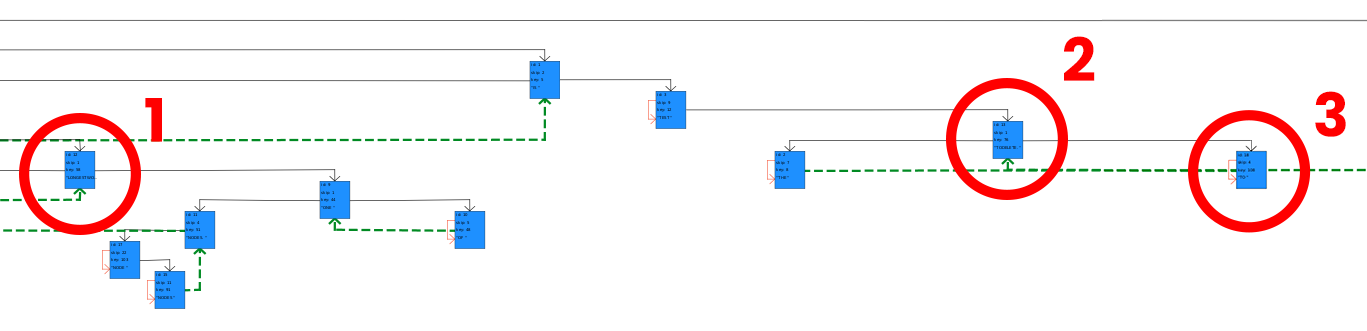
\includegraphics[width = \textwidth]{Delete1.png}
    	\end{figure}
    	
        \begin{figure}[htb]
    		\caption{Wizualizacja obiektu klasy \emph{PatriciaTree} stworzonego na podstawie pliku o zawartości ,,\texttt{THIS IS THE TEST FILE NUMBER 1 FOR DELETION ONE OF NODES. LONGESTWORDINTREExTODELETE. MORE NODES AFTER NODE TO DELETE;}``. Węzeł oznaczony liczbą 1 jest węzłem reprezentującym klucz ,,\texttt{LONGESTWORDINTREExTODELETE. }``. Węzeł oznaczony liczbą 3 jest węzłem reprezentującym klucz ,,\texttt{TO }``.}\label{fig:Delete2}
    		\centering
    		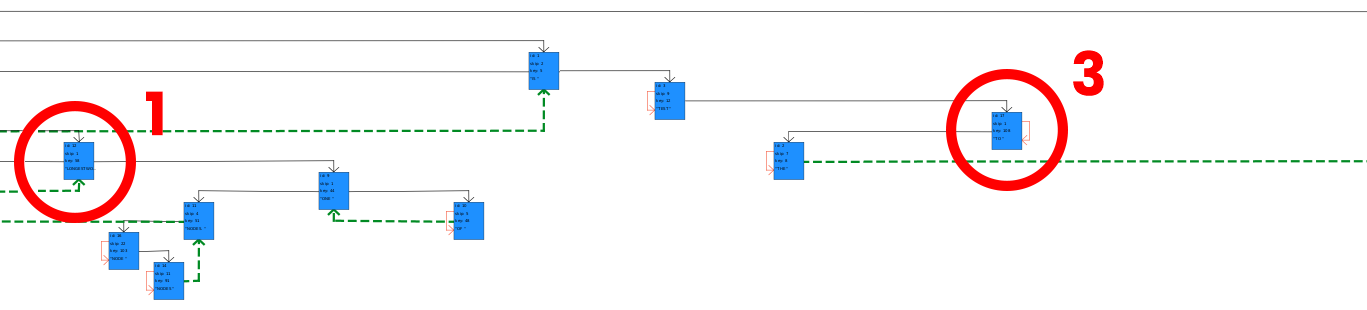
\includegraphics[width = \textwidth]{Delete2.png}
    	\end{figure}
		
		Knuth podczas omawiania algorytmów drzewa \emph{Patricia} wspomina jeszcze o możliwości dodawania nowych kluczy na końcu pliku poprzez wyznaczanie nowego unikatowego znaku końca pliku, który zamiast pojedynczego znaku miałby być starym znakiem końca pliku poprzedzonym liczbą tworzącym unikatowy ciąg znaków. Ta operacja również nie została zaimplementowana. Możliwe, że da się osiągnąć taki sam efekt w bardziej elegancki sposób. 
		
		\subsection{Autorska modyfikacja algorytmu drzewa \emph{Patricia}}\label{sec:RezultatyImplementacjiDrzewaPatriciaAutorska} 
	    
	    Odpowiedzią na tezę tego projektu inżynierskiego jest implementacja drzewa \emph{Patricia} w postaci klasy \emph{PatriciaTree} oraz możliwość wyboru strategii interpretacji tego czym jest klucz, dzięki parametrowi konstruktora typu \emph{enum} przyjmującym jedną z dwóch wartości: \emph{WordStrategy.START\textunderscore POSITION\textunderscore TO\textunderscore EOF} (odpowiadającej interpretacji Knuth'a tego czym jest klucz) lub \emph{WordStrategy.SINGLE} (mojej interpretacji, gdzie w skład każdego klucza nie wchodzą wszystkie klucze występujące po nim w pliku). 
	    
	    Zgodnie z opisem w sekcji~\ref{sec:czescPraktycznaImplementacjaDrzewaPatriciaAutorska}, modyfikacja algorytmów Donalda Knuth'a dotyczących drzewa \emph{Patricia} powiodła się. Dzięki dodaniu parametrów typu \emph{char} konstruktora klasy \emph{PatriciaTree}, określającego znak końca klucza modyfikacja ograniczała się w praktyce do stworzenia klasy implementującej oddzielny algorytm odczytywania klucza z pliku.
	    
	    Sprawdzenie rezultatów poprawności algorytmów wykonaliśmy za pomocą testów jednostkowych, opisanych w sekcji~\ref{sec:czescPraktycznaRezultatyImplementacjiTestyJednostkowe}. 
	    
	    Jednym z dowodów na brak znacznych modyfikacji względem algorytmów Knuth'a oraz struktury drzewa jest fakt, iż obie interpretacje tego czym jest klucz są dostępne w~jednej klasie \emph{PatriciaTree} -- a wybór ich odbywa się za pomocą wzorca projektowego strategia, który dostarcza jedną z klas dziedziczących po klasie \emph{FileOpsStrategy}. 
	    
	    Drugim dowodem na nieznaczny wpływ modyfikacji interpretacji tego czym jest klucz jest reprezentacja graficzna. Przykładowymi rysunkami przedstawiającymi przykład reprezentacji graficznej struktury drzewa dla takiej samej zawartości plików, ale różnej strategii pobierania klucza z pliku (interpretacji tego czym jest klucz) są rysunki ~\ref{fig:PatriciaTreeVisualRepresentation} i~\ref{fig:PatriciaTreeVisualRepresentationTest1}. 
	    
	    Dodatkową własnością, którą można zaobserwować na tych rysunkach jest fakt -- iż mimo oprócz różnych strategii te dwa obiekty korzystają z różnych kodowań znaków i~reprezentacji binarnych -- to struktura drzewa nie zmienia się w sposób znaczący. Różnicę w strukturze drzewa spowodowaną przez kodowanie znaków można zaobserwować dopiero na znakach wymagający do ich reprezentacji różnej ilości bajtów. Przykładami takich znaków są: $\theta$, $\Phi$, $\Pi$.
		
		\subsection{Koniunkcyjna postać normalna -- wykorzystanie autorskiej implementacji w rozwiązaniu problemu praktycznego}\label{sec:czescPraktycznaRezultatyCNF}
		
		Implementacja konwertera plików w formacie \emph{DIMCAS CNF} wykorzystuje klasę \emph{RandomAccessFile}, której obsługa została już napisana i wykorzystana wcześniej w programie projektowym. Niestety prędkość konwertowania pliku nie jest zadowalająca i może być to spowodowane właśnie wyborem klasy obsługującej pracę na plikach. Możliwe, że użycie kombinacji klas \emph{File}, \emph{FileReader}, \emph{BufferedReader} przez klasę \emph{CNFReader} (a przez klasę \emph{CNFWriter}: \emph{File}, \emph{FileWriter}, \emph{BufferedWriter}) skutkowałoby szybszym przetwarzaniem plików.
		
		Przykłady struktury klasy \emph{PatriciaTree} z klasy \emph{agh.jo.Examples} mają możliwość nie konwertowania plików poprzez ustawienie finalnego, statycznego pola \emph{DEFAULT\textunderscore IS\textunderscore DO\textunderscore CONVERT\textunderscore CNF\textunderscore SOURCE\textunderscore FILE\textunderscore TO\textunderscore PATRICIA\textunderscore SOURCE\textunderscore FILE} klasy \emph{App} na wartość \emph{false} dla przypadków kiedy nie nastąpiła zmiana pliku źródłowego \emph{CNF} i parametrów konstruktów klas \emph{PatriciaTree} i \emph{CNFConverter}.\newpage
		
		Jednym z wcześniej wspomnianych założeń upraszczających było założenie przyjęte przy konwertowaniu plików w formacie \emph{DIMACS CNF} dotyczące togo, że nie mogą się w nich pojawić dwie identyczne klauzule z punktu widzenia logiki Bool'a. Dzięki temu konwerter nie musi sprawdzać, czy klauzula wstawiana do pliku źródłowego drzewa już w~nim nie występuje. W efekcie implementacja drzewa \emph{Patricia} wyrzuca wyjątek mówiący o tym, że do struktury nie może zostać wstawiony klucz będący prefiksem już istniejącego~klucza.
		
		Kolejnym założeniem uproszczającym jest to, że każda klauzula w pliku \emph{DIMACS CNF} kończy się znakiem (lub kombinacją znaków) końca linii. Specyfikacja plików w~tym formacie mówi o przypadkach, w których może się zdarzyć, że dwie klauzule są w~tej samej linii, a rozdziela je ciąg znaków \emph{klauzula1 + `` 0 `` + klauzula2}. Specyfikacja mówi również o nieregularnych przypadkach, gdzie ostatnia klauzula w pliku nie jest zakończona kombinacją znaków \emph{ostatnia\textunderscore klauzula + `` 0``}. Dodatkowo dopuszczane są przypadki, w~których linie komentarzy przeplatają się z liniami klauzul.
		
		Następnym założeniem uproszczającym, niezwiązanym już ze specyfikacją plików w formacie \emph{DIMACS CNF}, jest wymóg klasy \emph{CNFConverter} istnienia pliku wejściowego i wyjściowego konwertera. Podobnie klasa \emph{PatriciaTree} wymaga istnienia pliku wejściowego, który jest plikiem wyjściowym konwertera. Zapobiega to sytuacji, w~której użytkownik mógłby popełnić błąd podając inne ścieżki czy nazwy plików dla tych dwóch klas i mógłby stanąć on przed zagadką ,,Dlaczego skoro konwerter poprawnie działa to klasa drzewa \emph{Patricia} wyrzuca wyjątek związany z brakiem pliku, który przecież konwerter \emph{NA PEWNO} tworzy? ``. Oczywiście nigdy się nie zdarzyło tak, żeby użytkownikiem w~takim scenariuszu byli autorzy tej pracy inżynierskiej -- czyli my.
		
		Z kolei wnioskiem wynikającym z zastosowania struktury jaką jest drzewo \emph{Patricia} do problemu plików zawierających koniunkcyjną postać normalną jest fakt, że nie jest ona kompatybilna z problemem. Drzewa typu \emph{Trie} korzystają z własności wynikających z kolejności ciągów znaków, podczas gdy klauzula, która jest alternatywą literałów -- nie dba o kolejność literałów. Dlatego do problemu, w którym kolejność wartości nie ma znaczenia lepszym wyborem były by \emph{hashowe}-funkcje (ang. \emph{hash-functions}). Inspiracją dla tego rozwiązania było przedstawienie ich praktycznego wykorzystania w wideo-artykule na przykładzie aplikacji \emph{Shazam} (aplikacji znajdującej nazwę utworu muzycznego na podstawie jego fragmentu rozpoznanego przez mikrofon telefonu) przez kanał \emph{RealEngineering} na \emph{YouTube}~\cite{HashFunctionsShazamYoutubeRealEngineering}.
		
		Dodatkowym problem, który dla ułatwienia ignorujemy jest fakt, że z logicznego punktu widzenia drzewa typu \emph{Trie} są alternatywą kluczy w nim w zawartych, podczas gdy koniunkcyjna postać normalna jest koniunkcją klauzul. Bardziej nadającym się do tego rozwiązania -- z tego punktu widzenia -- problemem jest problem \emph{DNF} (dysjunkcyjna postać normalna), który jest alternatywą koniunkcji literałów. \newpage Nie rozwiązuję to jednak problemu jakim jest dowolność kolejności literałów w~klauzulach alternatyw czy koniunkcji literałów.
		
		\subsection{Reprezentacja graficzna stworzonego drzewa}\label{sec:czescPraktycznaRezultatyImplementacjiReprezentacja graficzna}
		
		Dodanie reprezentacji graficznej jako dodatkowego elementu edukacyjnego oraz testowego zakończyło się sukcesem. Niekonwencjonalna budowa drzewa \emph{Patricia} -- a dokładniej -- orientacja węzłów względem siebie i gałęzi obrazujących relację tych węzłów -- wymagała autorskiej implementacji tworzenia wizualnej struktury drzewa. Niestety wymagało to dodania dodatkowych ,,ukrytych`` węzłów na gałęziach drzewa, aby było zrozumiałe z którego węzła wychodzi dana krawędź i do którego wchodzi. Spowodowało to, że obecnie zaimplementowana funkcjonalność przesuwania węzłów drzewa \emph{Patricia} w~czasie działania programu nie spełnia swojej funkcji, gdyż gałęzie zostają w pozycji startowej i niestety zaburza ona czytelność grafu. Decyzję czy warto reorganizować położenie węzłów drzewa \emph{Patricia} na grafie pozostawiam użytkownikowi.
		
		Jedynym ograniczeniem wizualizacji struktury klasy \emph{PatriciaTree} jest ilość krawędzi w drzewie -- bo na tym etapie przetwarzania program nie daje sobie rady z ilością wymaganej pamięci. Klasa \emph{PatriciaTreeVisualization} nie jest w stanie sobie poradzić ze strukturami klasy \emph{PatriciaTree} stworzonej na podstawie dwóch dużych plików o rozmiarze 1.5 i 8.4 Mb. Jest to dosyć ciekawy problem, którego rozwiązaniem nie może być po prostu zwiększenie ilości pamięci RAM przydzielonej programowi, gdyż zawsze może istnieć większy przykład drzewa \emph{Patricia}, wymagający większej ilości pamięci RAM. Rozwiązaniem tego problemu mogłoby być dynamiczne tworzenie i kasowanie obiektów odpowiednio widocznych i nie widocznych obecnie na ekranie oraz ograniczenie obszaru jaki może widzieć użytkownik korzystając z funkcjonalności oddalenia widoku. Inspiracją tego rozwiązania jest rozwiązanie popularnie stosowane w dzisiejszych grach, gdzie jedynie obiekty widoczne w następnej klatce są renderowane, a stare obiekty są niszczone na rzecz wolnej pamięci.
		
	\section{Możliwości rozwoju}\label{sec:podsumowanieMozliwosciRozwoju}
	
	Implementacja wykonana w zakresie tego projektu inżynierskiego w formie klasy \emph{PatriciaTree} jest uniwersalna i nadaje się do zastosowania przy problemach dużych zbiorów, których elementy mają określoną kolejność -- są ciągami liczb czy innych znaków. 
	
	Możliwością rozwoju samej implementacji postaci klasy \emph{PatriciaTree} jest implementacja operacji pominiętych w obecnej wersji (usuń, następca, poprzednik, minimum, maksimum). Dodatkowo można rozwinąć projekt o algorytmy umożliwiające modyfikację pliku źródłowego drzewa \emph{Patricia}. Takim algorytmem może być na przykład algorytm dodawania lub usuwania - do drzewa i jednocześnie pliku -- nowego klucza. Dokładniej opisany został ten problem w sekcji~\ref{sec:RezultatyImplementacjiDrzewaPatriciaKnuth}.
	
	Rozwojem rozważań tematu dotyczącego koniunkcyjnej postaci normalnej może być próba zastosowania \emph{hash}-funkcji do szybszego przeszukiwania zbioru klauzul. Dokładniej problem ten opisałem w sekcji~\ref{sec:czescPraktycznaRezultatyCNF}.
	
	Kolejną okazją do rozwoju tego projektu jest modyfikacja implementacji reprezentacji graficznej tak, aby niezależnie od rozmiaru drzewa \emph{Patricia}, generacja wizualnej warstwy projektu zawsze kończyła się sukcesem. Opis propozycji rozwiązania tego problemu opisałem w sekcji~\ref{sec:czescPraktycznaRezultatyImplementacjiReprezentacja graficzna}.